
\begin{frame}{Schéma E/A: la base des voyageurs}

\vspace*{0.3cm}

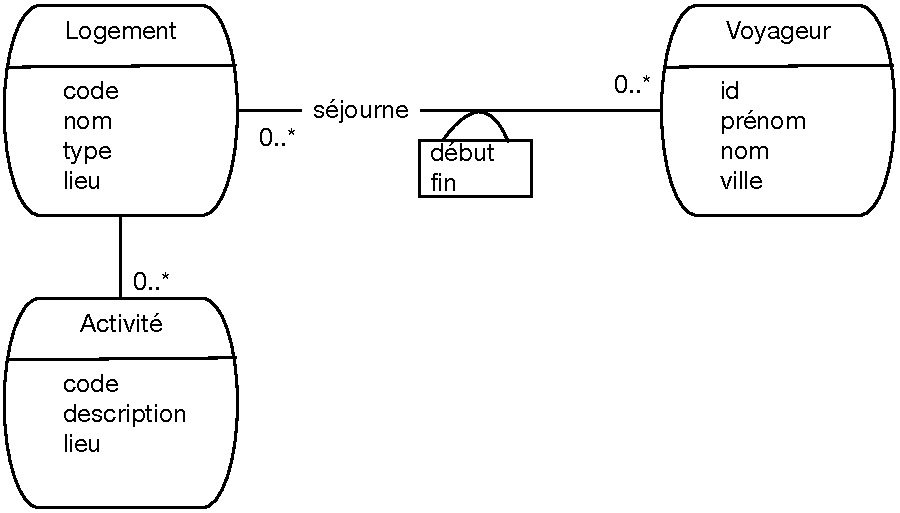
\includegraphics[width=8cm]{../figures-sql/schema-voyageurs}
\end{frame}


\begin{frame}{Les types d'entité}

\begin{center}
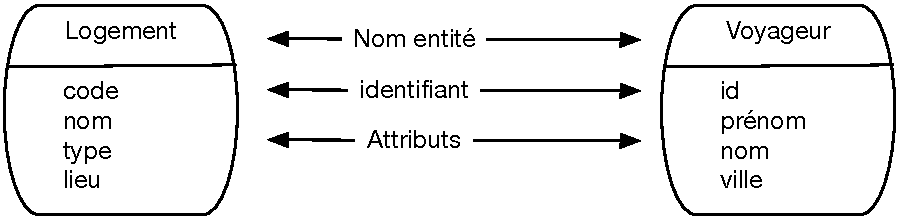
\includegraphics[width=10cm]{../figures-sql/type-entites}
\end{center}
\vfill

Un type d'entité représente une DF entre l'identifiant et les attributs

\vfill

\begin{redbullet}
  \item Tous les attributs sont \alert{atomiques}
  \item Choix de la clé: un attribut non-descriptif (\texttt{id}) est à peu près \alert{toujours}
      le meilleur choix.
\end{redbullet}

\end{frame}


\begin{frame}{Associations binaires}

Etudions l'association ``une activité a lieu dans un logement''

\vfill

\begin{center}
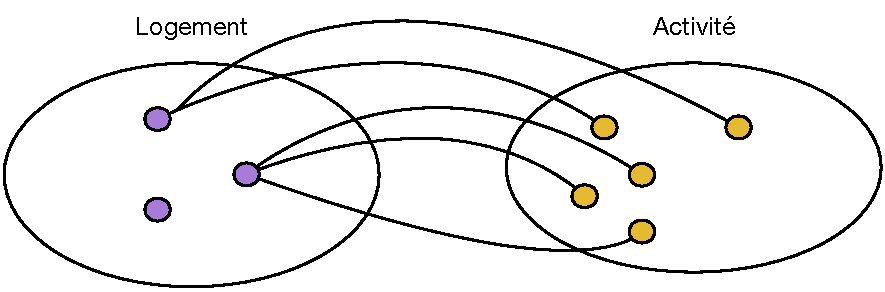
\includegraphics[width=8cm]{../figures-sql/graphe-activites}
\end{center}
\vfill

Décisions à prendre:

\begin{redbullet}
  \item La notion d'activité est-elle générique ou relative à un logement\,?
    \item Combien d'activités pour un logement, au plus, au moins\,?
\end{redbullet}

\end{frame}


\begin{frame}{Cardinalités}
Les choix de conception sont représentés par
des \alert{cardinalités}.

\vfill
Cardinalité de l'association pour $E$:
     une paire $[min, max]$  :


\begin{redbullet}
  \item $max$ (cardinalité maximale)\,:
       le nombre \alert{maximal} de fois où une 
      une entité $e$ de $E$  peut intervenir dans l'association (1 ou plusieurs).
      
    \item $min$  (cardinalité minimale),:
        le nombre \alert{minimal} de fois où une 
       une entité $e$ de $E$ peut intervenir dans l'association
       (0 ou 1)
\end{redbullet}

\vfill

Ces choix sont \alert{essentiels} (et difficiles à changer après coup).
\end{frame}


\begin{frame}{Association un-à-plusieurs (ou plusieurs-à-un)}

Représentation de l'association ``un logement propose  des activités''.

\vfill

\begin{center}
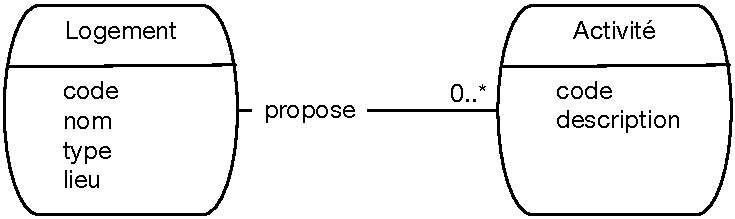
\includegraphics[width=8.5cm]{../figures-sql/association-activite}
\end{center}

\vfill
On a donc décidé qu'une activité est spécifique à un logement

\bigskip

On autorise qu'un logement ne propose pas d'activité

\end{frame}


\begin{frame}{À retenir}

Le modèle entité association
\vfill
\begin{redbullet}
  \item Entité: objets autonomes, identifiables, persistants.
 \item Associations: liens entre entités, caractérisées par des \alert{cardinalités}
\end{redbullet}

\vfill

Ne vise pas à représenter la réalité fidèlement ou complètement,
 mais en fonction d'un \alert{besoin}

\end{frame}

